% The bibliography travels inside this file: LaTeX writes smartlocker-refs.bib at compile time,
% so no separate .bib has to be uploaded (it is overwritten on every run).
\begin{filecontents*}[overwrite]{smartlocker-refs.bib}
@article{alfuqaha2015iot,
  author  = {Al-Fuqaha, Ala and Guizani, Mohsen and Mohammadi, Mehdi and Aledhari, Mohammed and Ayyash, Moussa},
  title   = {Internet of Things: A Survey on Enabling Technologies, Protocols, and Applications},
  journal = {IEEE Communications Surveys \& Tutorials},
  volume  = {17},
  number  = {4},
  pages   = {2347--2376},
  year    = {2015},
  doi     = {10.1109/COMST.2015.2444095},
  note    = {doi: 10.1109/COMST.2015.2444095}
}

@article{sicari2015security,
  author  = {Sicari, Sabrina and Rizzardi, Alessandra and Grieco, Luigi Alfredo and Coen-Porisini, Alberto},
  title   = {Security, Privacy and Trust in {Internet of Things}: The Road Ahead},
  journal = {Computer Networks},
  volume  = {76},
  pages   = {146--164},
  year    = {2015},
  doi     = {10.1016/j.comnet.2014.11.008},
  note    = {doi: 10.1016/j.comnet.2014.11.008}
}

@article{iwan2016parcel,
  author  = {Iwan, Stanis{\l}aw and Kijewska, Kinga and Lemke, Justyna},
  title   = {Analysis of Parcel Lockers' Efficiency as the Last Mile Delivery Solution: The Results of the Research in {Poland}},
  journal = {Transportation Research Procedia},
  volume  = {12},
  pages   = {644--655},
  year    = {2016},
  doi     = {10.1016/j.trpro.2016.02.018},
  note    = {doi: 10.1016/j.trpro.2016.02.018}
}

@article{mitrokotsa2010rfid,
  author  = {Mitrokotsa, Aikaterini and Rieback, Melanie R. and Tanenbaum, Andrew S.},
  title   = {Classifying {RFID} Attacks and Defenses},
  journal = {Information Systems Frontiers},
  volume  = {12},
  number  = {5},
  pages   = {491--505},
  year    = {2010},
  doi     = {10.1007/s10796-009-9210-z},
  note    = {doi: 10.1007/s10796-009-9210-z}
}

@article{chandola2009anomaly,
  author  = {Chandola, Varun and Banerjee, Arindam and Kumar, Vipin},
  title   = {Anomaly Detection: A Survey},
  journal = {ACM Computing Surveys},
  volume  = {41},
  number  = {3},
  pages   = {15:1--15:58},
  year    = {2009},
  doi     = {10.1145/1541880.1541882},
  note    = {doi: 10.1145/1541880.1541882}
}

@inproceedings{sommer2010outside,
  author    = {Sommer, Robin and Paxson, Vern},
  title     = {Outside the Closed World: On Using Machine Learning for Network Intrusion Detection},
  booktitle = {Proc. IEEE Symposium on Security and Privacy},
  pages     = {305--316},
  year      = {2010},
  doi       = {10.1109/SP.2010.25},
  note      = {doi: 10.1109/SP.2010.25}
}

@article{moustafa2021toniot,
  author  = {Moustafa, Nour},
  title   = {A New Distributed Architecture for Evaluating {AI}-Based Security Systems at the Edge: Network {TON\_IoT} Datasets},
  journal = {Sustainable Cities and Society},
  volume  = {72},
  pages   = {102994},
  year    = {2021},
  doi     = {10.1016/j.scs.2021.102994},
  note    = {doi: 10.1016/j.scs.2021.102994}
}

@article{hall2009weka,
  author  = {Hall, Mark and Frank, Eibe and Holmes, Geoffrey and Pfahringer, Bernhard and Reutemann, Peter and Witten, Ian H.},
  title   = {The {WEKA} Data Mining Software: An Update},
  journal = {ACM SIGKDD Explorations Newsletter},
  volume  = {11},
  number  = {1},
  pages   = {10--18},
  year    = {2009},
  doi     = {10.1145/1656274.1656278},
  note    = {doi: 10.1145/1656274.1656278}
}

@article{breiman2001rf,
  author  = {Breiman, Leo},
  title   = {Random Forests},
  journal = {Machine Learning},
  volume  = {45},
  number  = {1},
  pages   = {5--32},
  year    = {2001},
  doi     = {10.1023/A:1010933404324},
  note    = {doi: 10.1023/A:1010933404324}
}

@book{quinlan1993c45,
  author    = {Quinlan, J. Ross},
  title     = {C4.5: Programs for Machine Learning},
  publisher = {Morgan Kaufmann},
  address   = {San Mateo, CA},
  year      = {1993},
  isbn      = {1-55860-238-0},
  doi       = {10.1016/C2009-0-27846-9},
  note      = {doi: 10.1016/C2009-0-27846-9}
}

@inproceedings{john1995nb,
  author    = {John, George H. and Langley, Pat},
  title     = {Estimating Continuous Distributions in {Bayesian} Classifiers},
  booktitle = {Proc. 11th Conference on Uncertainty in Artificial Intelligence (UAI)},
  publisher = {Morgan Kaufmann},
  pages     = {338--345},
  year      = {1995},
  doi       = {10.48550/arXiv.1302.4964},
  note      = {doi: 10.48550/arXiv.1302.4964}
}

@article{aha1991ibl,
  author  = {Aha, David W. and Kibler, Dennis and Albert, Marc K.},
  title   = {Instance-Based Learning Algorithms},
  journal = {Machine Learning},
  volume  = {6},
  number  = {1},
  pages   = {37--66},
  year    = {1991},
  doi     = {10.1007/BF00153759},
  note    = {doi: 10.1007/BF00153759}
}

@inproceedings{kohavi1995cv,
  author    = {Kohavi, Ron},
  title     = {A Study of Cross-Validation and Bootstrap for Accuracy Estimation and Model Selection},
  booktitle = {Proc. 14th International Joint Conference on Artificial Intelligence (IJCAI)},
  volume    = {2},
  pages     = {1137--1144},
  year      = {1995},
  url       = {https://www.ijcai.org/proceedings/1995/147}
}

@article{haber1991timestamp,
  author  = {Haber, Stuart and Stornetta, W. Scott},
  title   = {How to Time-Stamp a Digital Document},
  journal = {Journal of Cryptology},
  volume  = {3},
  number  = {2},
  pages   = {99--111},
  year    = {1991},
  doi     = {10.1007/BF00196791},
  note    = {doi: 10.1007/BF00196791}
}

@inproceedings{provos1999bcrypt,
  author    = {Provos, Niels and Mazi{\`e}res, David},
  title     = {A Future-Adaptable Password Scheme},
  booktitle = {Proc. USENIX Annual Technical Conference, FREENIX Track},
  address   = {Monterey, CA},
  pages     = {81--92},
  year      = {1999},
  url       = {https://www.usenix.org/legacy/events/usenix99/provos.html}
}

@inproceedings{rfidiot2023locker,
  author    = {Bharatiraja, C. and Chittoor, Prithvi Krishna and Bhargava, Yash Vardhan},
  title     = {An {IoT} Based Centralized Smart Locker Using {RFID} Technology},
  booktitle = {AIP Conference Proceedings},
  volume    = {2427},
  number    = {1},
  pages     = {020098},
  publisher = {AIP},
  month     = feb,
  year      = {2023},
  doi       = {10.1063/5.0101139},
  note      = {doi: 10.1063/5.0101139}
}

@article{roman2013features,
  author  = {Roman, Rodrigo and Zhou, Jianying and Lopez, Javier},
  title   = {On the Features and Challenges of Security and Privacy in Distributed {Internet of Things}},
  journal = {Computer Networks},
  volume  = {57},
  number  = {10},
  pages   = {2266--2279},
  year    = {2013},
  doi     = {10.1016/j.comnet.2012.12.018},
  note    = {doi: 10.1016/j.comnet.2012.12.018}
}

@article{abomhara2015cyber,
  author  = {Abomhara, Mohamed and K{\o}ien, Geir M.},
  title   = {Cyber Security and the {Internet of Things}: Vulnerabilities, Threats, Intruders and Attacks},
  journal = {Journal of Cyber Security and Mobility},
  volume  = {4},
  number  = {1},
  pages   = {65--88},
  year    = {2015},
  doi     = {10.13052/jcsm2245-1439.414},
  note    = {doi: 10.13052/jcsm2245-1439.414}
}

@article{want2006rfid,
  author  = {Want, Roy},
  title   = {An Introduction to {RFID} Technology},
  journal = {IEEE Pervasive Computing},
  volume  = {5},
  number  = {1},
  pages   = {25--33},
  year    = {2006},
  doi     = {10.1109/MPRV.2006.2},
  note    = {doi: 10.1109/MPRV.2006.2}
}

@article{coskun2013nfc,
  author  = {Coskun, Vedat and Ozdenizci, Busra and Ok, Kerem},
  title   = {A Survey on Near Field Communication ({NFC}) Technology},
  journal = {Wireless Personal Communications},
  volume  = {71},
  number  = {3},
  pages   = {2259--2294},
  year    = {2013},
  doi     = {10.1007/s11277-012-0935-5},
  note    = {doi: 10.1007/s11277-012-0935-5}
}

@article{jain2004biometric,
  author  = {Jain, Anil K. and Ross, Arun and Prabhakar, Salil},
  title   = {An Introduction to Biometric Recognition},
  journal = {IEEE Transactions on Circuits and Systems for Video Technology},
  volume  = {14},
  number  = {1},
  pages   = {4--20},
  year    = {2004},
  doi     = {10.1109/TCSVT.2003.818349},
  note    = {doi: 10.1109/TCSVT.2003.818349}
}

@article{ahmed2016survey,
  author  = {Ahmed, Mohiuddin and Mahmood, Abdun Naser and Hu, Jiankun},
  title   = {A Survey of Network Anomaly Detection Techniques},
  journal = {Journal of Network and Computer Applications},
  volume  = {60},
  pages   = {19--31},
  year    = {2016},
  doi     = {10.1016/j.jnca.2015.11.016},
  note    = {doi: 10.1016/j.jnca.2015.11.016}
}

% ---------------------------------------------------------------------------------------------
% New works, 2022 to 2025 (each checked on the publisher page and on Crossref, 2026-11-14).
% ---------------------------------------------------------------------------------------------

@article{zhang2025parcel,
  author  = {Zhang, Qiruo and Demir, Emrah},
  title   = {Parcel Locker Solutions for Last Mile Delivery: A Systematic Literature Review and Future Research Directions},
  journal = {Frontiers in Future Transportation},
  volume  = {6},
  pages   = {1654621},
  month   = aug,
  year    = {2025},
  doi     = {10.3389/ffutr.2025.1654621},
  note    = {doi: 10.3389/ffutr.2025.1654621}
}

@article{ciesla2023parcel,
  author  = {Cie{\'s}la, Maria},
  title   = {Perceived Importance and Quality Attributes of Automated Parcel Locker Services in Urban Areas},
  journal = {Smart Cities},
  volume  = {6},
  number  = {5},
  pages   = {2661--2679},
  month   = oct,
  year    = {2023},
  doi     = {10.3390/smartcities6050120},
  note    = {doi: 10.3390/smartcities6050120}
}

@article{demedeiros2023anomaly,
  author  = {DeMedeiros, Kyle and Hendawi, Abdeltawab and Alvarez, Marco},
  title   = {A Survey of {AI}-Based Anomaly Detection in {IoT} and Sensor Networks},
  journal = {Sensors},
  volume  = {23},
  number  = {3},
  pages   = {1352},
  month   = jan,
  year    = {2023},
  doi     = {10.3390/s23031352},
  note    = {doi: 10.3390/s23031352}
}

@article{shahin2025twostage,
  author  = {Shahin, Mohammad and Hosseinzadeh, Ali and Chen, F. Frank},
  title   = {A Two-Stage Hybrid Federated Learning Framework for Privacy-Preserving {IoT} Anomaly Detection and Classification},
  journal = {IoT},
  volume  = {6},
  number  = {3},
  pages   = {48},
  year    = {2025},
  doi     = {10.3390/iot6030048},
  note    = {doi: 10.3390/iot6030048}
}

@article{arp2024pitfalls,
  author  = {Arp, Daniel and Quiring, Erwin and Pendlebury, Feargus and Warnecke, Alexander and Pierazzi, Fabio and Wressnegger, Christian and Cavallaro, Lorenzo and Rieck, Konrad},
  title   = {Pitfalls in Machine Learning for Computer Security},
  journal = {Communications of the ACM},
  volume  = {67},
  number  = {11},
  pages   = {104--112},
  month   = nov,
  year    = {2024},
  doi     = {10.1145/3643456},
  note    = {doi: 10.1145/3643456}
}
\end{filecontents*}

\documentclass[journal,onecolumn]{IEEEtran}
\usepackage{cite}
\usepackage{amsmath,amssymb,amsfonts}
\usepackage{graphicx}
\usepackage{textcomp}
\usepackage{float}
\usepackage{array}
\usepackage{iftex}
\ifPDFTeX
  \usepackage[T1]{fontenc}
  \usepackage[utf8]{inputenc}
  \usepackage{newtxtext,newtxmath}
\else
  \usepackage{fontspec}
  \setmainfont{TeX Gyre Termes}[
    Extension = .otf,
    UprightFont = *-regular,
    BoldFont = *-bold,
    ItalicFont = *-italic,
    BoldItalicFont = *-bolditalic
  ]
\fi
\usepackage{tikz}
% Shared TikZ setup for the figures of the paper (figs/fig-*.tex).
% Light pastel fills, dark borders and black text; no purple and no gray anywhere.
% Every style and colour is prefixed with "sl" so nothing clashes with the paper's own preamble.
% The figures are drawn at their natural size (at most 17.5 cm, \linewidth is 18.1 cm in the
% one-column IEEEtran layout), so the \small labels print at 9 pt without any scaling.
\usetikzlibrary{arrows.meta,positioning,fit,shapes.geometric,calc,backgrounds}

% pastel fills
\definecolor{slBlue}{HTML}{DCEBFA}    % light blue: clients, entry points
\definecolor{slMint}{HTML}{DDF3E3}    % mint green: server, processing
\definecolor{slYellow}{HTML}{FFF3C4}  % pale yellow: decisions, services
\definecolor{slPeach}{HTML}{FFE2C8}   % peach: hardware outputs, data access
\definecolor{slCoral}{HTML}{FFD9D6}   % light coral/pink: alerts, outcomes
\definecolor{slSky}{HTML}{E9F6FB}     % very light cyan: group backgrounds
% dark borders (one per fill) and ink
\definecolor{slBlueD}{HTML}{1F4E79}
\definecolor{slMintD}{HTML}{1E6B3A}
\definecolor{slYellowD}{HTML}{7A5B00}
\definecolor{slPeachD}{HTML}{8A4513}
\definecolor{slCoralD}{HTML}{9B2226}
\definecolor{slInk}{HTML}{0F2338}     % arrows and lines (dark navy)

\tikzset{
  % basic block: one main line of text; \slsub{...} adds an optional smaller second line
  slbox/.style={draw=slBlueD, fill=slBlue, rounded corners=3pt, line width=0.7pt, align=center,
                font=\small, text=black, inner xsep=5pt, inner ysep=4pt, minimum height=0.8cm},
  slblue/.style={slbox},
  slmint/.style={slbox, draw=slMintD, fill=slMint},
  slyellow/.style={slbox, draw=slYellowD, fill=slYellow},
  slpeach/.style={slbox, draw=slPeachD, fill=slPeach},
  slcoral/.style={slbox, draw=slCoralD, fill=slCoral},
  sldec/.style={draw=slYellowD, fill=slYellow, diamond, aspect=2.1, line width=0.7pt, align=center,
                font=\small, text=black, inner sep=1pt},
  slterm/.style={slbox, draw=slCoralD, fill=slCoral, line width=1.0pt},
  slok/.style={slbox, draw=slMintD, fill=slMint, line width=1.0pt},
  % arrows end exactly on the node border (default anchors, no shortening)
  slarr/.style={draw=slInk, line width=0.8pt, -{Latex[length=2.4mm, width=1.7mm]}},
  sldbl/.style={draw=slInk, line width=0.8pt, {Latex[length=2.4mm, width=1.7mm]}-{Latex[length=2.4mm, width=1.7mm]}},
  slret/.style={slarr, dashed},
  sllbl/.style={font=\small, text=black, inner sep=2pt},
  slbus/.style={font=\footnotesize, text=slInk, fill=white, inner sep=1.5pt},
  slgroup/.style={draw=slMintD, dashed, rounded corners=5pt, line width=0.7pt},
  slgrouplbl/.style={font=\small\bfseries, text=slMintD, inner sep=2pt},
}
% smaller second line inside a block
\newcommand{\slsub}[1]{\\[-1pt]{\footnotesize #1}}

\usetikzlibrary{arrows.meta,positioning,fit,shapes.geometric}
\tikzset{every picture/.style={line width=0.6pt}}
% pack figures and tables tightly (the paper has many floats)
\renewcommand{\topfraction}{0.9}
\renewcommand{\bottomfraction}{0.8}
\renewcommand{\textfraction}{0.07}
\renewcommand{\floatpagefraction}{0.85}
\setcounter{topnumber}{3}
\setcounter{bottomnumber}{2}
\setcounter{totalnumber}{5}
\setlength{\textfloatsep}{10pt plus 2pt minus 2pt}
\setlength{\floatsep}{8pt plus 2pt minus 2pt}
\setlength{\intextsep}{8pt plus 2pt minus 2pt}
% the commit on which code counts, tests and measurements were taken (Section VI-A)
\newcommand{\measurecommit}{13ba35f} % CHECK-FINAL: set to the final commit

\begin{document}

\title{Smart Locker with Anomalous Access Detection Based on IoT Device Telemetry}

\author{%
\begin{tabular}{ccc}
Duc Hoang Nguyen & Viet Tien Nguyen & Huy Hoang Nguyen \\
{\small duchoang.nguyen103@fpt.edu.vn} & {\small tiennv@fpt.edu.vn} & {\small hoangnh@fpt.edu.vn} \\[8pt]
Thanh Cao Nguyen & Thu Le & Kieu Trong Khanh$^{*}$ \\
{\small thanhnc@fpt.edu.vn} & {\small thulvm@fpt.edu.vn} & {\small khanhkt@fpt.edu.vn} \\[8pt]
\multicolumn{3}{c}{FPT University, Ho Chi Minh Campus, Vietnam} \\[2pt]
\multicolumn{3}{c}{\small $^{*}$Corresponding author}
\end{tabular}}

\maketitle

\begin{abstract}
Shared lockers on university campuses are still opened with mechanical keys or paper codes, cannot be reserved,
and give staff no view of forced doors, lost cards or forgotten items; once networked, their unlock signal can also be
forged or replayed. This paper presents SmartLocker, a locker rental system in which users reserve a slot on a web map,
pay from a prepaid wallet and open it with a personal identification number (PIN), a radio-frequency identification
(RFID) card, a fingerprint or a phone page. The ESP32 box takes no access decision: it forwards every credential to the
server, which replies \texttt{UNLOCK} or \texttt{DENY}. Abnormal access is detected mainly by a priority-ordered rule
engine over device telemetry and server context, which recognises sensor faults, spoofed remote opens, lost cards,
forced opening, wrong-user access, items left behind and overdue storage. A machine-learning risk score is kept only as
a secondary signal and raises an alert for sessions that no rule explains. On synthetic labelled sessions, the best of
four Weka classifiers made almost all of its errors between wrong-user and normal sessions, which share the same
telemetry by construction; identity is therefore checked by rule, and the score should be trusted only once real
sessions are available. All automated tests and replayed detection scenarios passed, and the server answered every % CHECK-FINAL: all tests passed
device request within about 0.1~s.
\end{abstract}

\begin{IEEEkeywords}
Smart locker, Internet of Things, ESP32, RFID, anomaly detection, rule engine, machine learning, Weka.
\end{IEEEkeywords}

\section{Introduction}

\IEEEPARstart{S}{elf-service} lockers are now common for parcels and short-term storage in campuses, canteens, gyms
and libraries \cite{iwan2016parcel}. Most of the lockers found on campuses, however, are purely mechanical: a key or a
code on paper opens the door, a slot cannot be booked before the user arrives, and the operator has no record of what
happens at the box. A forced door, a lost card picked up by someone else or belongings left for several days are
discovered only when somebody reports them. The Internet of Things (IoT) \cite{alfuqaha2015iot} makes the state of
every slot visible to a server, but it also brings the classic weaknesses of connected devices: a box can be
impersonated, an unlock message can be forged or replayed, and sensor readings can be wrong or manipulated
\cite{sicari2015security, roman2013features}. A shared campus facility therefore requires both a convenient reservation
and rental service and automated access monitoring that safeguards unattended personal property.

SmartLocker addresses both the rental service and these threats for a shared campus locker. We treat the box as a thin,
authenticated client and let the server take every decision, since only the server holds the full context of a
booking, and the resulting contributions are listed in Table~\ref{tab:contrib}. The priority-ordered rule tier of the
detector is the main contribution; the machine-learning risk score is kept as a secondary signal, because it has so far
been trained on synthetic data only. Section~II reviews related work, Section~III describes the system design,
Section~IV the detection method and Section~V the implementation. Section~VI reports the evaluation and Section~VII
concludes the paper.

\begin{table}[!htbp]
\renewcommand{\arraystretch}{1.15}
\centering
\small
\caption{Contributions of This Work and Where They Are Shown}
\label{tab:contrib}
\begin{tabular}{c p{11.6cm} p{3.0cm}}
\hline
No. & Contribution & Where it is shown \\
\hline
1 & A complete locker rental system with reservation on a map, prepaid payment, four opening methods (PIN, RFID card,
    fingerprint and phone) and an ESP32 box that only forwards credentials signed with a per-device key; all money and
    time rules run in database transactions. & Sections III and V \\
2 & A priority-ordered rule engine over device telemetry and server context that labels sensor faults, spoofed remote
    opens, lost cards, forced opening, wrong-user access, items left behind and overdue storage, completed by
    server-side safeguards and a hash-chained audit log, with a machine-learning risk score as a secondary signal for
    sessions that no rule explains. & Section IV \\
3 & An evaluation with automated tests, replayed detection scenarios and server response times, and a comparison of
    four classifiers on synthetic data showing that telemetry alone cannot separate wrong-user from normal access. &
    Section VI \\
\hline
\end{tabular}
\end{table}

\section{Related Work}

\textit{Smart and parcel lockers.} Research on parcel lockers has concentrated on last-mile logistics, where lockers
reduce failed deliveries and courier trips \cite{iwan2016parcel}, rather than on access security. A recent systematic
review finds the same focus: most studies of locker networks optimise locker locations and delivery routes, and only
one of the sustainability studies it classifies deals with safety and security \cite{zhang2025parcel}. On the user
side, a survey of parcel locker users in Poland ranks a dedicated application, a box size matched to the item and the
location of the stations among the most important quality attributes of the service \cite{ciesla2023parcel}. An IoT
locker based on RFID \cite{rfidiot2023locker} identifies the user with an identity card and uses Wi-Fi to monitor the
locker, log accesses and watch for unauthorised use. SmartLocker answers the needs of users with booking on a map and
slot sizes that are priced separately, and it adds prepaid payment, several credentials and a detector that raises
typed alerts instead of only recording accesses.

\textit{Security of IoT devices and credentials.} Surveys of IoT security list impersonation, message spoofing and
physical tampering among the main threats to constrained devices \cite{abomhara2015cyber} and recommend that trust be
established on the server side \cite{sicari2015security}. RFID \cite{want2006rfid} is exposed to cloning, replay and
relay attacks \cite{mitrokotsa2010rfid}, and near field communication (NFC) readers inherit these risks
\cite{coskun2013nfc}. Biometric credentials such as fingerprints tie access to a person instead of a token, but they
require a trusted matcher \cite{jain2004biometric}. SmartLocker follows these recommendations by keeping every access
decision on the server and by identifying each box with a secret key of which only a hash is stored. Distributed and
federated architectures have also been studied to preserve the privacy of user telemetry while aggregating security
insights across nodes \cite{shahin2025twostage}.

\textit{Anomaly detection.} Rule-based, statistical and learned detectors are the three families usually distinguished
in surveys of anomaly detection \cite{chandola2009anomaly, ahmed2016survey}. For IoT and sensor networks, a survey of
recent detectors finds that most are learned models such as multilayer perceptrons, recurrent networks and
autoencoders, that the detection of malicious actors is their most common application, and that the scarcity of
labelled data makes fully supervised detectors less successful than unsupervised ones \cite{demedeiros2023anomaly}.
Like SmartLocker, Shahin et al. \cite{shahin2025twostage} detect in two tiers: a generative model trained on the benign
traffic of each device flags anomalous IoT traffic, and a gradient-boosting classifier then labels the flagged traffic,
with an average accuracy of 99.14\% on the N-BaIoT dataset. For intrusion detection, Sommer and Paxson
\cite{sommer2010outside} show that learned detectors are hard to interpret, raise costly false alarms and work best on
narrow, well-understood problems, and a later analysis of 30 machine-learning papers from top security venues finds
that each one suffers from at least three of ten common pitfalls, among them sampling bias and lab-only evaluation
\cite{arp2024pitfalls}. SmartLocker has no labelled sessions from real use yet, so its first tier is a set of explicit
rules over device telemetry and booking context on the server, and its learned model only adds a risk score as
supporting evidence. The classifiers are trained with Weka
\cite{hall2009weka}, the audit log follows the hash-chaining scheme of Haber and Stornetta \cite{haber1991timestamp},
and passwords are stored with BCrypt \cite{provos1999bcrypt}.

\section{System Design}

\subsection{Architecture}

SmartLocker has a three-tier architecture (Fig.~\ref{fig:arch}). The clients are web browsers used by end users and
staff, a phone unlock page and the ESP32 locker box. The application tier is a Java 8 Servlet/JSP application that
follows the MVC2 pattern on Apache Tomcat~9, and the data tier is a SQL Server database that also implements the
business rules as stored procedures. In the end-to-end workflow (Fig.~\ref{fig:workflow}), credentials and telemetry
are captured at the box and forwarded to the server, which takes the access decision and runs the detector. Every
outcome is stored as a booking change, an alert or an audit entry and can then be reviewed by staff or by the user.
Door time and weight enter this workflow from the device simulator for now, because the prototype box has no door
sensor or load cell yet.

\begin{figure}[!htbp]
\centering
% Fig. 1 (fig:arch): three-tier architecture. Needs figs/colors.tex. Natural width about 17 cm.
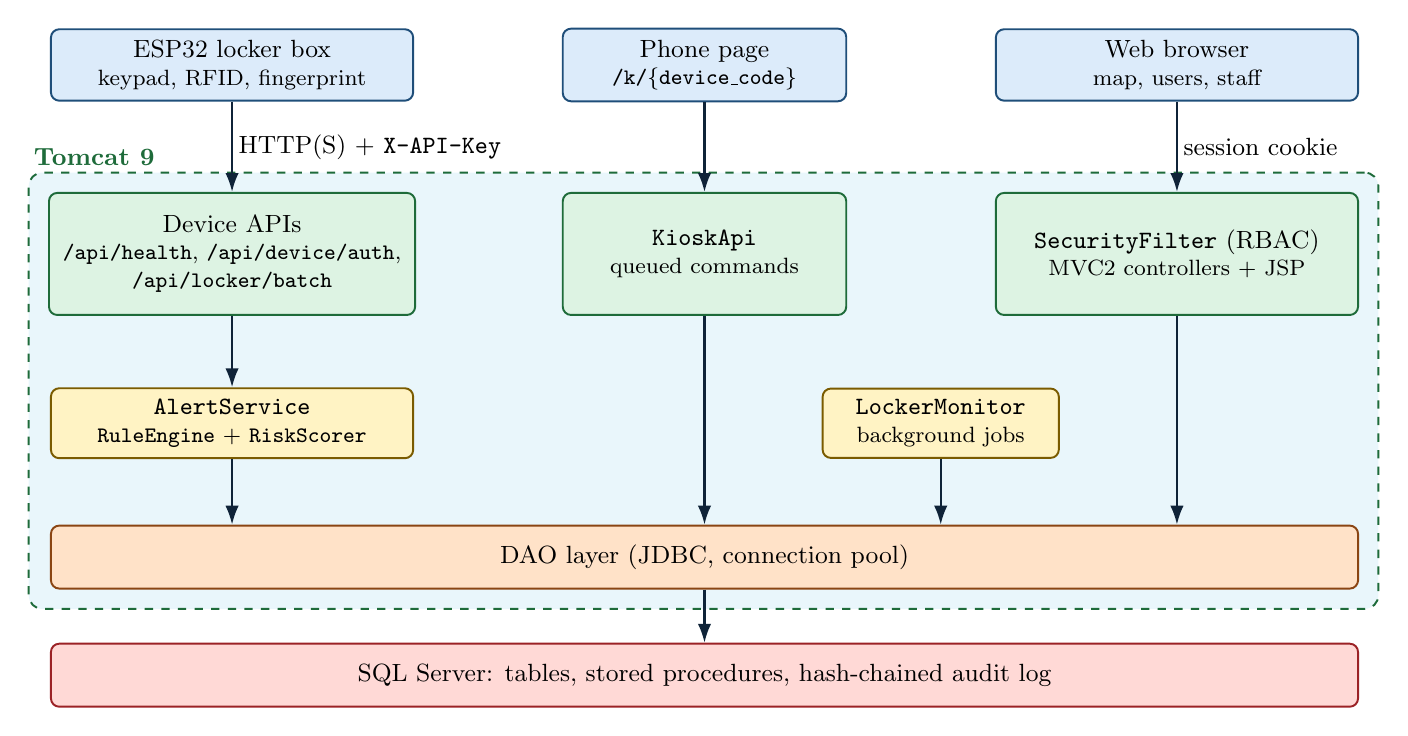
\begin{tikzpicture}
  % clients (top row)
  \node[slblue, minimum width=4.6cm] (esp)   at (2.4,4.3)  {ESP32 locker box\slsub{keypad, RFID, fingerprint}};
  \node[slblue, minimum width=3.6cm] (phone) at (8.4,4.3)  {Phone page\slsub{\texttt{/k/\{device\_code\}}}};
  \node[slblue, minimum width=4.6cm] (web)   at (14.4,4.3) {Web browser\slsub{map, users, staff}};
  % application tier
  \node[slmint, minimum width=4.6cm, minimum height=1.55cm] (devapi) at (2.4,1.9)
       {Device APIs\slsub{\texttt{/api/health}, \texttt{/api/device/auth},}\slsub{\texttt{/api/locker/batch}}};
  \node[slmint, minimum width=3.6cm, minimum height=1.55cm] (kiosk) at (8.4,1.9)
       {\texttt{KioskApi}\slsub{queued commands}};
  \node[slmint, minimum width=4.6cm, minimum height=1.55cm] (ctrl) at (14.4,1.9)
       {\texttt{SecurityFilter} (RBAC)\slsub{MVC2 controllers + JSP}};
  \node[slyellow, minimum width=4.6cm] (svc) at (2.4,-0.25) {\texttt{AlertService}\slsub{\texttt{RuleEngine} + \texttt{RiskScorer}}};
  \node[slyellow, minimum width=3.0cm] (mon) at (11.4,-0.25) {\texttt{LockerMonitor}\slsub{background jobs}};
  \node[slpeach, minimum width=16.6cm] (dao) at (8.4,-1.95) {DAO layer (JDBC, connection pool)};
  % data tier
  \node[slcoral, minimum width=16.6cm] (db) at (8.4,-3.45) {SQL Server: tables, stored procedures, hash-chained audit log};
  % arrows: client to entry point
  \draw[slarr] (esp)   -- node[sllbl, right] {HTTP(S) + \texttt{X-API-Key}} (devapi);
  \draw[slarr] (phone) -- (kiosk);
  \draw[slarr] (web)   -- node[sllbl, right] {session cookie} (ctrl);
  % arrows inside Tomcat, all straight down onto the DAO layer
  \draw[slarr] (devapi) -- (svc);
  \draw[slarr] (svc)    -- (svc |- dao.north);
  \draw[slarr] (kiosk)  -- (kiosk |- dao.north);
  \draw[slarr] (mon)    -- (mon |- dao.north);
  \draw[slarr] (ctrl)   -- (ctrl |- dao.north);
  \draw[slarr] (dao)    -- (db);
  % Tomcat container drawn behind the blocks
  \begin{scope}[on background layer]
    \node[slgroup, fill=slSky, fit=(devapi)(kiosk)(ctrl)(svc)(mon)(dao), inner xsep=7pt, inner ysep=7pt,
          label={[slgrouplbl, anchor=south west]north west:Tomcat 9}] (tc) {};
  \end{scope}
\end{tikzpicture}

\caption{Three-tier architecture of SmartLocker, in which the ESP32 box, the phone page and the web browser reach the
Tomcat application through separate entry points and every outcome is stored in SQL Server.}
\label{fig:arch}
\end{figure}

\begin{figure}[!htbp]
\centering
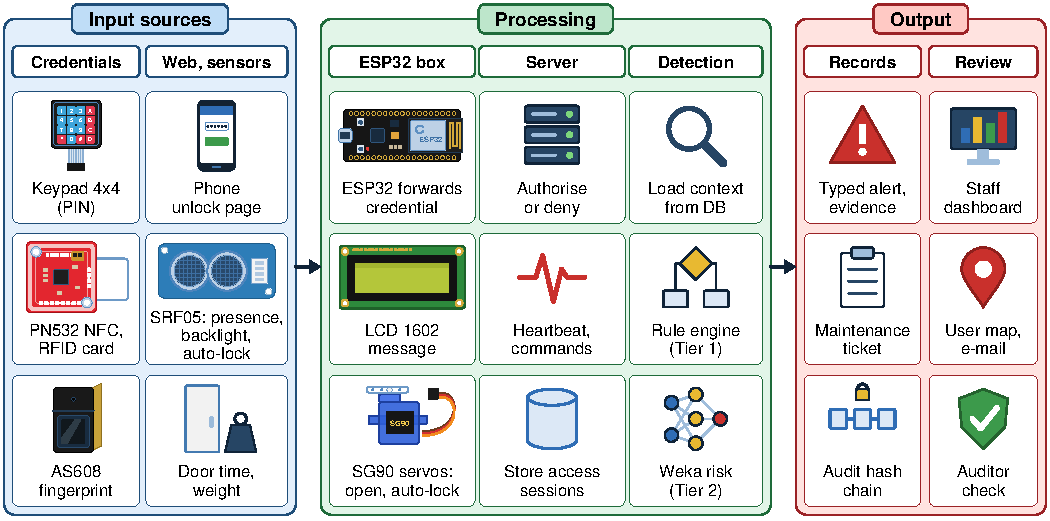
\includegraphics[width=\linewidth]{images/workflow.pdf}
\caption{Workflow of SmartLocker from input sources through processing to output, with hardware drawn after the
prototype box and with door time and weight taken from the device simulator because the box has no door sensor or load
cell yet.}
\label{fig:workflow}
\end{figure}

\subsection{Roles}

Access to the web application is governed by role-based access control (RBAC) with five roles: \texttt{END\_USER}
(book, pay, open, extend, cancel, top up), \texttt{OPERATOR} (remote open, top-up approval, areas, banks, slots,
plans, cards, bookings), \texttt{TECHNICIAN} (alerts, maintenance, calibration), \texttt{AUDITOR} (read-only access,
audit-chain verification) and \texttt{ADMIN} (everything, including roles and permissions). Visitors may browse the map
without an account, but booking, profile management and payment require an active session. Write endpoints inspect the
role of the authenticated caller before executing business logic, and unauthorized operations are blocked at the filter
boundary. All administrative and operational actions are permanently recorded in the audit log to prevent privilege
abuse. The box authenticates with its own per-device key, ensuring that device API requests are bound to the specific
physical hardware.

\subsection{Data Model}

Lockers are organised in three levels: an \emph{area} is a pin on the map (Leaflet, or Mapbox GL when a token is
configured), a \emph{bank} is a column of lockers controlled by one device, and a \emph{slot} has size S
($20\times20\times20$~cm), M ($40\times40\times40$~cm) or L ($60\times60\times60$~cm). A booking is a row of
\texttt{Deposit} linking a user, a slot, a plan and optionally a card, and filtered unique indexes reject a second open
booking for the same slot or user. Access sessions are append-only, enforced by an update and delete database trigger
that preserves raw sensor measurements. Alerts retain evidence rows for operational diagnostics, and remote commands
record when they were issued, sent and completed. Monetary balances and wallet deductions are executed solely within
transactions that apply exclusive locks to eliminate race conditions.

\subsection{Hardware}

The locker box is built around an ESP32 development board (Table~\ref{tab:hw} and Fig.~\ref{fig:block}). A 4$\times$4
keypad reads PINs and menu keys, a PN532 NFC reader reads RFID cards, an AS608 optical sensor reads fingerprints, a
16$\times$2 I$^2$C LCD displays messages, and two servos drive the bolt and the door. An SRF05 ultrasonic sensor
detects a person in front of the box, switches on the LCD backlight and locks the door 20~s after the person has left,
or at the latest 120~s after opening; pressing D on the keypad locks it at once. A regulated 5~V power supply powers the
servos and sensors, while decoupling capacitors stabilize the supply rail against voltage dips caused by motor inrush
current. The box sends a heartbeat every 3~s and executes the commands contained in the reply.

\begin{table}[!htbp]
\renewcommand{\arraystretch}{1.1}
\centering
\small
\caption{Hardware Components of the Locker Box}
\label{tab:hw}
\begin{tabular}{l l l}
\hline
Component & Function & ESP32 pins \\
\hline
ESP32 Dev Module & Controller, Wi-Fi, HTTP(S) client & Built-in \\
PN532 & RFID card reader (I$^2$C, 0x24) & SDA 21, SCL 22 (shared with LCD) \\
AS608 & Fingerprint sensor (UART) & TX$\rightarrow$35, RX 15 \\
LCD 1602 I$^2$C & User messages & SDA 21, SCL 22 \\
Keypad 4$\times$4 & PIN and menu input & Rows 13, 14, 25, 26; columns 33, 19, 23, 27 \\
Servo (bolt / door) & Locks the slot / opens the door & 32 / 2 \\
SRF05 & Presence detection (backlight, automatic lock) & TRIG 5, ECHO 18 \\
\hline
\end{tabular}
\end{table}

\begin{figure}[!htbp]
\centering
% Fig. 3 (fig:block): block diagram of the prototype box (firmware 4.3) and the server. Needs figs/colors.tex.
% SRF05 role from firmware/SmartLocker_Online (4.3): presence wakes the LCD backlight, and the door locks
% DOOR_OPEN_MS = 20 s after the last person left, or DOOR_OPEN_MAX_MS = 120 s after opening at the latest.
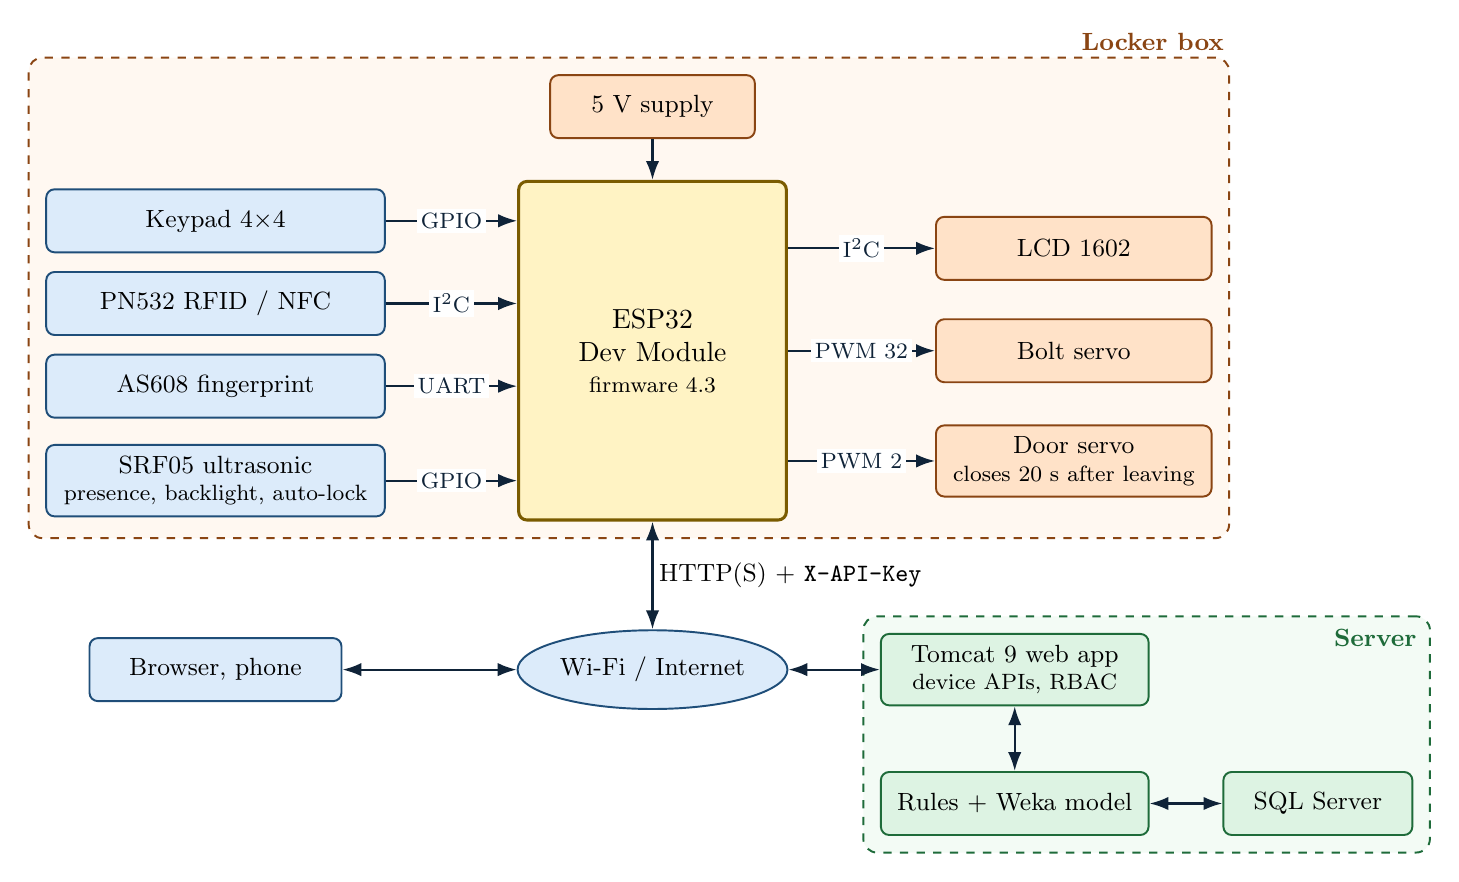
\begin{tikzpicture}
  % inputs (left)
  \node[slblue, minimum width=4.3cm] (kp) at (2.15,1.65)  {Keypad 4$\times$4};
  \node[slblue, minimum width=4.3cm] (rf) at (2.15,0.6)   {PN532 RFID / NFC};
  \node[slblue, minimum width=4.3cm] (fp) at (2.15,-0.45) {AS608 fingerprint};
  \node[slblue, minimum width=4.3cm] (us) at (2.15,-1.65) {SRF05 ultrasonic\slsub{presence, backlight, auto-lock}};
  % controller
  \node[slyellow, line width=1.1pt, minimum width=3.4cm, minimum height=4.3cm, font=\normalsize] (esp) at (7.7,0)
       {ESP32\\Dev Module\slsub{firmware 4.3}};
  \node[slpeach, minimum width=2.6cm] (pw) at (7.7,3.1) {5~V supply};
  % outputs (right)
  \node[slpeach, minimum width=3.5cm] (lcd) at (13.05,1.3)  {LCD 1602};
  \node[slpeach, minimum width=3.5cm] (sb)  at (13.05,0)    {Bolt servo};
  \node[slpeach, minimum width=3.5cm] (sd)  at (13.05,-1.4) {Door servo\slsub{closes 20~s after leaving}};
  % wires
  \draw[slarr] (kp.east) -- node[slbus] {GPIO} (kp.east -| esp.west);
  \draw[slarr] (rf.east) -- node[slbus] {I$^2$C} (rf.east -| esp.west);
  \draw[slarr] (fp.east) -- node[slbus] {UART} (fp.east -| esp.west);
  \draw[slarr] (us.east) -- node[slbus] {GPIO} (us.east -| esp.west);
  \draw[slarr] (pw) -- (esp);
  \draw[slarr] (lcd.west -| esp.east) -- node[slbus] {I$^2$C} (lcd.west);
  \draw[slarr] (sb.west -| esp.east)  -- node[slbus] {PWM 32} (sb.west);
  \draw[slarr] (sd.west -| esp.east)  -- node[slbus] {PWM 2} (sd.west);
  % network, clients and server (bottom)
  \node[draw=slBlueD, fill=slBlue, ellipse, line width=0.7pt, font=\small, align=center, inner sep=1pt,
        minimum width=2.9cm, minimum height=1.0cm] (net) at (7.7,-4.05) {Wi-Fi / Internet};
  \node[slblue, minimum width=3.2cm] (cl) at (2.15,-4.05) {Browser, phone};
  \node[slmint, minimum width=3.4cm] (tc) at (12.3,-4.05) {Tomcat 9 web app\slsub{device APIs, RBAC}};
  \node[slmint, minimum width=3.4cm] (ml) at (12.3,-5.75) {Rules + Weka model};
  \node[slmint, minimum width=2.4cm] (db) at (16.15,-5.75) {SQL Server};
  \draw[sldbl] (esp) -- node[sllbl, right] {HTTP(S) + \texttt{X-API-Key}} (net);
  \draw[sldbl] (cl) -- (net);
  \draw[sldbl] (net) -- (tc);
  \draw[sldbl] (tc) -- (ml);
  \draw[sldbl] (ml) -- (db);
  \begin{scope}[on background layer]
    \node[slgroup, draw=slPeachD, fill=slPeach!25, fit=(kp)(us)(pw)(esp)(lcd)(sd), inner sep=6pt,
          label={[slgrouplbl, text=slPeachD, anchor=south east]north east:Locker box}] {};
    \node[slgroup, fill=slMint!35, fit=(tc)(ml)(db), inner sep=6pt,
          label={[slgrouplbl, anchor=north east, inner sep=5pt]north east:Server}] {};
  \end{scope}
\end{tikzpicture}

\caption{Block diagram of the prototype box, in which the ESP32 reads the keypad, the card and fingerprint readers and
the SRF05 sensor, drives the LCD and the two servos, and reaches the server over Wi-Fi.}
\label{fig:block}
\end{figure}

\subsection{Device Protocol}

Each box holds a secret API key; the database stores only its SHA-256 hash, and the server derives the device
identity from the key, never from the request body. Three endpoints carry the protocol (two more enrol cards and
fingerprints):
\begin{itemize}
  \item \texttt{POST /api/health}: heartbeat every 3~s, whose reply carries pending commands (remote
        \texttt{UNLOCK}, fingerprint deletion) and the blocked card UIDs.
  \item \texttt{POST /api/device/auth}: a PIN, card UID or fingerprint slot with an \emph{intent} (\texttt{ASK},
        \texttt{OPEN}, \texttt{CHECKOUT}), answered by \texttt{UNLOCK}, \texttt{CHOOSE}, \texttt{CONFIRM\_EMAIL} or
        \texttt{DENY} with a reason and the attempts left.
  \item \texttt{POST /api/locker/batch}: buffered access sessions with a per-device sequence number, so a session sent
        again after an outage is stored once.
\end{itemize}
The current firmware does not upload sessions yet, so the batch endpoint is exercised by a device simulator
(Section~VI). A box may control several banks; the \texttt{physical} flag of \texttt{UNLOCK} moves the servo only for
the wired slot. Because a lost card can be used by anyone, a card scan is confirmed by its owner when the server can
send e-mail: the box receives \texttt{CONFIRM\_EMAIL}, and the server releases a held \texttt{UNLOCK} (valid for
5~minutes) after a POST on a single-use link, stored only as a hash, or after a confirmation on the map. A card
presented at the wrong box is refused with \texttt{WRONG\_PLACE}, which names the correct bank. An opening at the box
is answered at once, whereas a remote or phone open reaches the box with its next heartbeat and comes back as a session
carrying the command identifier (Fig.~\ref{fig:seq}).

\begin{figure}[!htbp]
\centering
% Fig. 4 (fig:seq): sequence of the device protocol. Needs figs/colors.tex. Natural width about 17.3 cm.
% Solid arrows are requests, dashed arrows are replies; every arrow starts and ends on a lifeline.
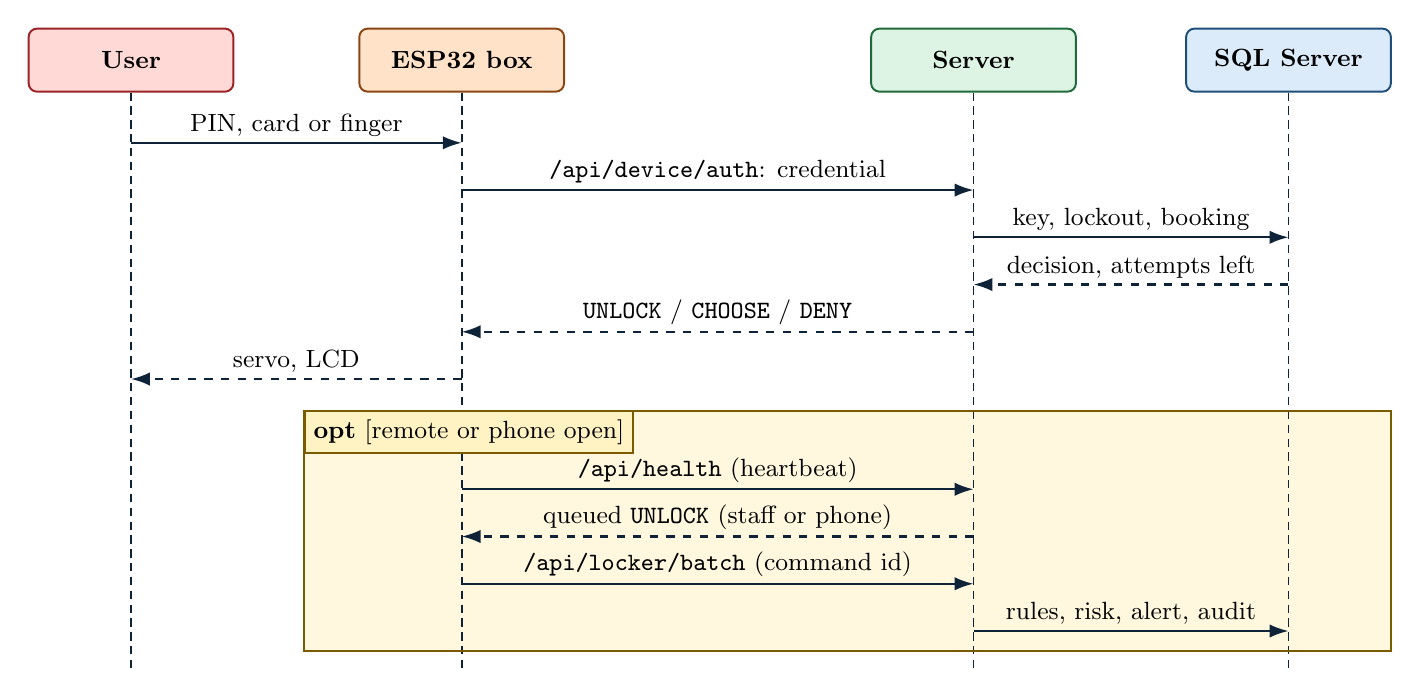
\begin{tikzpicture}[
  head/.style={minimum width=2.6cm, font=\small\bfseries},
  t/.style={sllbl, above, inner sep=2pt}]
  \def\xU{1.3}\def\xE{5.5}\def\xS{12.0}\def\xD{16.0}\def\yEnd{-7.75}
  % fill of the opt fragment first, so that the lifelines and arrows are drawn over it
  \fill[slYellow!55] (3.5,-4.45) rectangle (17.3,-7.5);
  % lifelines
  \node[slcoral, head] (u) at (\xU,0) {User};
  \node[slpeach, head] (e) at (\xE,0) {ESP32 box};
  \node[slmint,  head] (s) at (\xS,0) {Server};
  \node[slblue,  head] (d) at (\xD,0) {SQL Server};
  \foreach \n/\x in {u/\xU, e/\xE, s/\xS, d/\xD}
    \draw[draw=slInk, densely dashed, line width=0.6pt] (\n.south) -- (\x,\yEnd);
  % frame and tag of the opt fragment, over the lifelines
  \draw[draw=slYellowD, line width=0.7pt] (3.5,-4.45) rectangle (17.3,-7.5);
  \node[draw=slYellowD, fill=slYellow, line width=0.7pt, font=\small, anchor=north west, inner sep=3pt]
       at (3.5,-4.45) {\textbf{opt} [remote or phone open]};
  % opening at the box
  \draw[slarr] (\xU,-1.05) -- node[t] {PIN, card or finger} (\xE,-1.05);
  \draw[slarr] (\xE,-1.65) -- node[t] {\texttt{/api/device/auth}: credential} (\xS,-1.65);
  \draw[slarr] (\xS,-2.25) -- node[t] {key, lockout, booking} (\xD,-2.25);
  \draw[slret] (\xD,-2.85) -- node[t] {decision, attempts left} (\xS,-2.85);
  \draw[slret] (\xS,-3.45) -- node[t] {\texttt{UNLOCK} / \texttt{CHOOSE} / \texttt{DENY}} (\xE,-3.45);
  \draw[slret] (\xE,-4.05) -- node[t] {servo, LCD} (\xU,-4.05);
  % remote or phone open, carried by the heartbeat
  \draw[slarr] (\xE,-5.45) -- node[t] {\texttt{/api/health} (heartbeat)} (\xS,-5.45);
  \draw[slret] (\xS,-6.05) -- node[t] {queued \texttt{UNLOCK} (staff or phone)} (\xE,-6.05);
  \draw[slarr] (\xE,-6.65) -- node[t] {\texttt{/api/locker/batch} (command id)} (\xS,-6.65);
  \draw[slarr] (\xS,-7.25) -- node[t] {rules, risk, alert, audit} (\xD,-7.25);
\end{tikzpicture}

\caption{Sequence of the device protocol for an opening at the box (top) and a remote or phone open inside a UML
\emph{opt} fragment (bottom), with requests drawn as solid arrows and replies as dashed arrows.}
\label{fig:seq}
\end{figure}

\subsection{Booking Lifecycle}

A reservation charges the wallet and holds the slot for 15~minutes (Fig.~\ref{fig:state}); cancelling within
5~minutes refunds 100\% and later during the hold 50\%. Opening the slot during the hold is a \texttt{CHECK\_IN}, which
starts the paid time; if nobody comes, the booking starts by itself when the hold ends (\texttt{AUTO\_CHECK\_IN}) and
the slot stays locked for its owner, with nothing refunded. A booking that was never opened ends at its due time plus
the grace period as a \texttt{NO\_SHOW} without a late fee, and three no-shows within the last 7~days block new bookings
until the oldest no-show is more than 7~days old. Later authentications offer ``A: Open / B: Checkout'', where A keeps the
rental (\texttt{ACCESS}) and B ends it (\texttt{PICKUP}), and a booking can be extended three times. An overdue booking
that was opened is never released, since the belongings are still inside: after the grace period of the plan (15~minutes
for hourly plans and 30~minutes for the day pass) the slot is \emph{locked}, every late hour costs 150\% of the hourly rate,
the box refuses to open (\texttt{OVERDUE\_UNPAID}) until the debt is paid, and after 48~hours an \texttt{OVERDUE\_ESCALATED}
alert goes to staff.

\begin{figure}[!htbp]
\centering
% Fig. 5 (fig:state): states of a locker slot. Needs figs/colors.tex. Natural width about 17.2 cm.
% Since sql/05_auto_checkin.sql (v7.1) a reservation that nobody checks in starts by itself at the end of the
% 15-minute hold (AUTO_CHECK_IN); it is no longer freed as a no-show. A booking that was never opened ends as
% NO_SHOW at due time + grace, which frees the slot.
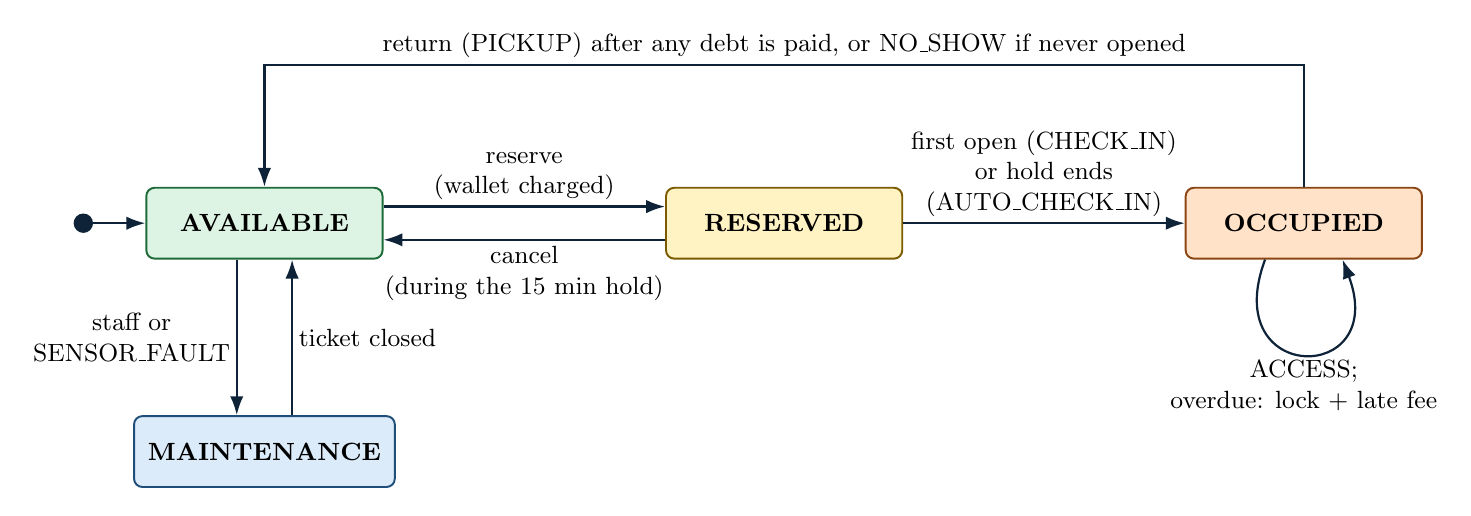
\begin{tikzpicture}[
  st/.style={minimum width=3.0cm, minimum height=0.9cm, font=\small\bfseries},
  lbl/.style={sllbl, align=center}]
  \node[slmint,   st] (av) at (0,0)     {AVAILABLE};
  \node[slyellow, st] (re) at (6.6,0)   {RESERVED};
  \node[slpeach,  st] (oc) at (13.2,0)  {OCCUPIED};
  \node[slblue,   st] (mt) at (0,-2.9)  {MAINTENANCE};
  % initial state
  \fill[slInk] (-2.3,0) circle (3.5pt);
  \draw[slarr] (-2.18,0) -- (av);
  % reserve and cancel: two parallel arrows, labels outside them
  \draw[slarr] ([yshift=6pt]av.east) -- node[lbl, above] {reserve\\(wallet charged)} ([yshift=6pt]re.west);
  \draw[slarr] ([yshift=-6pt]re.west) -- node[lbl, below] {cancel\\(during the 15 min hold)} ([yshift=-6pt]av.east);
  \draw[slarr] (re) -- node[lbl, above] {first open (CHECK\_IN)\\or hold ends\\(AUTO\_CHECK\_IN)} (oc);
  % the return runs above every label
  \draw[slarr] (oc.north) -- ++(0,1.55) -| node[lbl, above, pos=0.25]
       {return (PICKUP) after any debt is paid, or NO\_SHOW if never opened} (av.north);
  \draw[slarr] ([xshift=-14pt]oc.south) .. controls +(-0.6,-1.6) and +(0.6,-1.6) .. node[lbl, below]
       {ACCESS;\\overdue: lock + late fee} ([xshift=14pt]oc.south);
  \draw[slarr] ([xshift=-10pt]av.south) -- node[lbl, left] {staff or\\SENSOR\_FAULT} ([xshift=-10pt]mt.north);
  \draw[slarr] ([xshift=10pt]mt.north) -- node[lbl, right] {ticket closed} ([xshift=10pt]av.south);
\end{tikzpicture}

\caption{States of a locker slot starting from AVAILABLE (filled dot), where an overdue booking stays ACTIVE and keeps
its slot OCCUPIED until the debt is paid.}
\label{fig:state}
\end{figure}

\section{Anomalous Access Detection}

\subsection{Access Sessions and Context}

Each opening of a slot produces an \emph{access session} described by five features, uploaded through
\texttt{/api/locker/batch}: the door time (how long the door stayed open, in seconds), the weight change inside the
slot (in grams), the number of unlock events, whether a valid RFID card was read, and the stay time (how long the items
remained in the slot, in minutes). A session also records the source of the opening (local, remote or phone), the card UID
and, for a remote open, the identifier of the command. Telemetry alone does not reveal \emph{who} opened the slot, so
before deciding the server loads the context of the session from the database: the status and owner of the card, the owner
of the active booking, whether the remote command was actually issued and is still unused, the stay allowed by the plan,
the valid range of each sensor, the validity of the weight calibration, and the offset between the device clock and
the server clock. The five features form the feature vector $\mathbf{x}_s$ used by the machine-learning risk model, while
the context fields are evaluated exclusively by the rule engine. A session retransmitted after a network disconnection is
stored only once, because the batch endpoint enforces deduplication using the per-device sequence number.

\subsection{Tier 1: Priority-Ordered Rule Engine}

The rules of Table~\ref{tab:rules} are evaluated in a fixed order and the first matching rule determines the label.
The order is essential: readings from a faulty sensor must not be reported as a break-in, and a legitimate remote open
by staff must not be reported as a forced opening. The valid sensor ranges (door 0 to 3600~s, weight $-200$ to
20\,000~g, stay 0 to 10\,080~min) are stored in the database, so they can be adjusted without redeploying the
application. Rule 2' represents the negative branch of rule 2 and therefore occupies the same priority rank in the
evaluation sequence. Rules 4 to 8 then classify physical slot events, arranged strictly from the most critical security
violations to lower-severity operational exceptions.

\begin{table}[!htbp]
\renewcommand{\arraystretch}{1.1}
\centering
\small
\caption{Detection Rules in Priority Order}
\label{tab:rules}
\begin{tabular}{c l p{8.4cm} l}
\hline
\# & Label & Condition & Action \\
\hline
1 & SENSOR\_FAULT & door time, weight change or stay time outside the sensor's valid range; door open longer than the whole stay; device clock more than 300~s ahead of the server; weight calibration expired & Alert, ticket, no ML \\
2 & STAFF\_OPEN & remote or phone open with a valid, unused command for this slot, issued at most 30~min before the session (a box clock up to 60~s behind is tolerated) & Command done, no alert \\
2' & SUSPECTED\_SPOOF & remote or phone open without a valid command (never issued, or already used) & Alert \\
3 & LOST\_CARD\_USED & the card is not active (reported lost or blocked) & Alert \\
4 & FORCED\_OPEN & the door opened although no valid card was read & Alert \\
5 & WRONG\_USER & a valid card whose owner is not the owner of the booking & Alert \\
6 & SUSPECTED\_SPOOF & the weight changed by more than 50~g while the door reported ``never opened'' & Alert \\
7 & ITEM\_LEFT & the weight in the slot grew by more than 50~g (items left after pick-up) & Alert \\
8 & OVERDUE & stay time longer than the plan allows & Alert \\
9 & NORMAL & no rule matched & Tier 2 \\
\hline
\end{tabular}
\end{table}

\subsection{Tier 2: Machine-Learning Risk Score}

Let $\mathbf{x}_s = (d, w, u, v, t)$ denote the five features of a session $s$ (door time, weight change, unlocks,
valid card and stay time). A classifier trained offline on labelled sessions estimates the probability that $s$ is
normal, and the \emph{risk score} is defined as
\begin{equation}
r(s) = 1 - P\left(y = \text{NORMAL} \mid \mathbf{x}_s\right).
\label{eq:risk}
\end{equation}
The training tool compares four classifiers (Section~VI) and deploys the six-class model with the highest weighted F1,
which is currently IBk ($k=5$); for a hand-made session with normal-looking telemetry it yields $r = 0.20$. Let
$\ell(s)$ be the label of the first rule of Table~\ref{tab:rules} that matches $s$. The alert raised for $s$ is then
\begin{equation}
A(s) =
\begin{cases}
\ell(s), & \ell(s) \neq \text{NORMAL},\\
\text{ML\_ANOMALY}, & \ell(s) = \text{NORMAL} \text{ and } r(s) \geq \tau,\\
\text{none}, & \text{otherwise},
\end{cases}
\label{eq:alert}
\end{equation}
with the threshold $\tau = 0.80$; when a rule matches, $r(s)$ is stored with its alert as evidence. Without a
deployed model the risk is zero, and it is never computed for SENSOR\_FAULT or STAFF\_OPEN. A STAFF\_OPEN marks its
command as done through a conditional update, so of two sessions carrying the same command only one is a staff open and
the other becomes SUSPECTED\_SPOOF. A SENSOR\_FAULT also takes the slot out of service and opens a maintenance ticket
(one per device), and commands and alerts are written to the audit chain, following the decision flow of
Fig.~\ref{fig:flow}.

\begin{figure}[!htbp]
\centering
% Fig. 6 (fig:flow): decision flow of the two-tier detector for one session. Needs figs/colors.tex.
% Laid out across the page width (about 17.2 cm). Decisions are yellow diamonds; outcomes have a thick border:
% coral when an alert is raised, mint when no alert is raised.
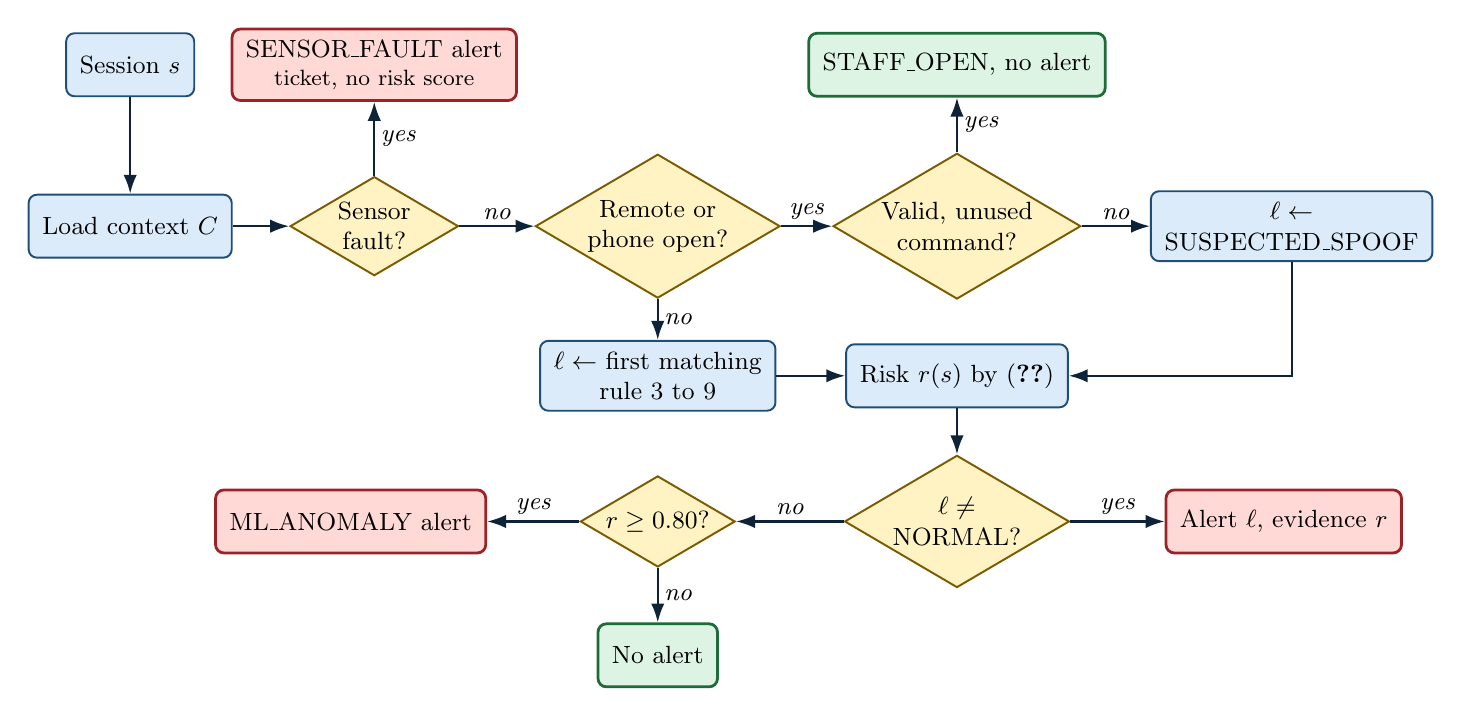
\begin{tikzpicture}[
  proc/.style={slblue},
  dec/.style={sldec, aspect=1.7},
  yes/.style={sllbl, font=\small\itshape},
  no/.style={sllbl, font=\small\itshape}]
  % row 1: input, context and the first two decisions, left to right
  \node[proc]  (in)  at (1.2,2.05)  {Session $s$};
  \node[proc]  (ctx) at (1.2,0)     {Load context $C$};
  \node[dec]   (sf)  at (4.3,0)     {Sensor\\fault?};
  \node[dec]   (rem) at (7.9,0)     {Remote or\\phone open?};
  \node[dec]   (cmd) at (11.7,0)    {Valid, unused\\command?};
  \node[proc]  (spf) at (15.95,0)    {$\ell \leftarrow$\\SUSPECTED\_SPOOF};
  % outcomes above row 1
  \node[slterm] (flt) at (4.3,2.05)  {SENSOR\_FAULT alert\slsub{ticket, no risk score}};
  \node[slok]   (stf) at (11.7,2.05) {STAFF\_OPEN, no alert};
  % row 2: rules 3 to 9 and the risk score
  \node[proc]  (rul) at (7.9,-1.9)  {$\ell \leftarrow$ first matching\\rule 3 to 9};
  \node[proc]  (rsk) at (11.7,-1.9) {Risk $r(s)$ by (\ref{eq:risk})};
  % row 3: the alert decision of (2), right to left
  \node[dec]   (lab) at (11.7,-3.75) {$\ell \neq$\\NORMAL?};
  \node[slterm] (ar) at (15.85,-3.75) {Alert $\ell$, evidence $r$};
  \node[dec]   (thr) at (7.9,-3.75)  {$r \geq 0.80$?};
  \node[slterm] (am) at (4.0,-3.75)  {ML\_ANOMALY alert};
  \node[slok]  (non) at (7.9,-5.45)   {No alert};
  % arrows
  \draw[slarr] (in) -- (ctx);
  \draw[slarr] (ctx) -- (sf);
  \draw[slarr] (sf) -- node[yes, right] {yes} (flt);
  \draw[slarr] (sf) -- node[no, above] {no} (rem);
  \draw[slarr] (rem) -- node[yes, above] {yes} (cmd);
  \draw[slarr] (rem) -- node[no, right] {no} (rul);
  \draw[slarr] (cmd) -- node[yes, right] {yes} (stf);
  \draw[slarr] (cmd) -- node[no, above] {no} (spf);
  \draw[slarr] (rul) -- (rsk);
  \draw[slarr] (spf) |- (rsk);
  \draw[slarr] (rsk) -- (lab);
  \draw[slarr] (lab) -- node[yes, above] {yes} (ar);
  \draw[slarr] (lab) -- node[no, above] {no} (thr);
  \draw[slarr] (thr) -- node[yes, above] {yes} (am);
  \draw[slarr] (thr) -- node[no, right] {no} (non);
\end{tikzpicture}

\caption{Decision flow of the two-tier detector for one access session, in which the rules of Table~\ref{tab:rules}
run first and the risk score of (\ref{eq:risk}) raises an ML\_ANOMALY alert only when no rule matched, as in
(\ref{eq:alert}), with outcomes drawn as boxes with a thick border, coral when an alert is raised and mint otherwise.}
\label{fig:flow}
\end{figure}

\subsection{Server-Side Safeguards}

Credential guessing, silent devices, lost cards, cards at the wrong box and overdue storage need no telemetry, because
the server state alone reveals them.
\begin{itemize}
  \item \textit{Credential guessing.} Every wrong PIN, unknown card or unknown finger counts towards a lockout: five
        wrong guesses within 5~minutes lock the box for 120~s; the phone page has its own counter (five tries,
        2~minutes).
  \item \textit{Silent devices.} A job running every 15~s marks a box without heartbeat for more than 90~s as
        \texttt{OFFLINE}, raises \texttt{DEVICE\_OFFLINE} and stops bookings on its banks.
  \item \textit{Lost cards} are pushed to the box in the blocked list of the next heartbeat (\texttt{CARD\_BLOCKED}).
  \item \textit{Card at the wrong box.} \texttt{WRONG\_PLACE} is logged on the booking the card was meant for, shown
        on the owner's map and e-mailed at most once per 10~minutes; it is not counted as a guess.
  \item \textit{Overdue storage} is locked, charged and escalated after 48~hours with its evidence.
\end{itemize}

\subsection{Tamper-Evident Audit Log}

Every business action and alert is appended to an audit log whose entries store the SHA-256 hash of their fields
(identifier, time, actor, action, object, change) and the hash of the previous entry \cite{haber1991timestamp}. The
hash chain starts from a well-known genesis entry initialized during database setup, forming an unbroken cryptographic
record. The last entry is read under an update lock, so concurrent writers cannot fork the chain, and changing or
deleting an entry breaks every later hash. Auditors inspect the hash consistency through an administrative interface,
and an automated background thread re-verifies the entire chain every 60~s to detect unauthorized modifications.

\section{Implementation}

% CHECK-FINAL: recount on the final commit: find src/java -name '*.java' | wc -l (89), physical lines of those files
% (11 736), find web -name '*.jsp' | wc -l (22); the UI translation may change them.
The server is written in Java~8 (about 11\,700 lines, comments and blank lines included, in 89 source files) with
22 JSP views and uses Gson, jBCrypt \cite{provos1999bcrypt} and Weka \cite{hall2009weka}. The interface is in English,
while technical codes such as slot codes, card UIDs and status values are shown as they are. It loads no script from a
content delivery network (Leaflet and Mapbox GL are bundled) and offers light and dark themes; when map tiles cannot be
loaded, the pins are drawn over a plain grid. The web interface follows responsive design principles and is compatible with
both desktop monitors and mobile phone browsers. Static assets and client-side templates are cached locally to minimize
bandwidth consumption during repeated campus visits.

\textit{Business rules in the database.} Every rule involving money or time (reservation, refund, extension,
overdue fee, escalation) is a stored procedure. Procedures that read and then modify a row lock it with
\texttt{UPDLOCK, HOLDLOCK} inside the transaction, so a slot cannot be booked twice and an extension cannot be charged
twice. The price of a plan is multiplied by a size factor (S 100\%, M 130\%, L 169\%) and rounded up to 100~VND
(Table~\ref{tab:price}); the late fee is 150\% of the unrounded hourly rate derived from the 2-hour plan, rounded once,
which is why size M pays 4\,900~VND and not 1.5 times 3\,300~VND. Users may also book 1 to 23 whole hours at the hourly
rate, capped at the day pass, or 1 to 7 whole days (90\% of the day pass per day for 2 to 6 days, 80\% for 7 days).
All opening methods cost the same.

\begin{table}[!htbp]
\renewcommand{\arraystretch}{1.1}
\centering
\small
\caption{Prices by Plan and Slot Size (VND)}
\label{tab:price}
\begin{tabular}{l r r r}
\hline
Plan & S & M & L \\
\hline
2 hours & 5\,000 & 6\,500 & 8\,500 \\
4 hours & 9\,000 & 11\,700 & 15\,300 \\
Day pass & 25\,000 & 32\,500 & 42\,300 \\
Hourly rate (extension) & 2\,500 & 3\,300 & 4\,300 \\
Late fee per hour (150\%) & 3\,800 & 4\,900 & 6\,400 \\
\hline
\end{tabular}
\end{table}

\textit{Monitoring and user interface.} A background thread (\texttt{LockerMonitor}) rebuilds an in-memory dashboard
snapshot every 2~s, so polling dashboards never query the database, and runs the expiry procedures every 15~s. Two more
threads re-verify the audit chain every 60~s and send due reminders by e-mail 15~minutes before a booking ends. Users
reserve and open slots from the map and the booking page (Fig.~\ref{fig:ui-user}), while staff follow devices, revenue
and alerts from the dashboard (Fig.~\ref{fig:ui-staff}). The booking confirmation states the amount taken now and the
refund and late-fee rules before the wallet is charged, and an escalated alert keeps the evidence of the late booking
for the operator. All devices except LOCKER-01 are demo devices whose heartbeat is simulated by the server, so the
demo areas stay online without hardware.

\textit{Security.} Passwords are hashed with BCrypt, and device keys are stored only as SHA-256 hashes. The session
user is reloaded from the database on every request, so a locked account is signed out at once. A failed sign-in is
logged with the account name only if that account exists. All user data is escaped, using \texttt{<c:out>} in JSP
templates and a single centralized escaping function in JavaScript. Visitors may open only the map and its read-only
public data, and every state-modifying request requires an authenticated session.

% CHECK-FINAL: ui-user/ui-staff (2026-11-14) still show the Vietnamese UI; retake them in English and recheck every
% number in both captions (23 of 27, B07, 6 500 VND, 11 alerts, 10 of 10, #119, A12, 50 h, 320 000 / 128 500 VND)
\begin{figure}[!htbp]
\centering
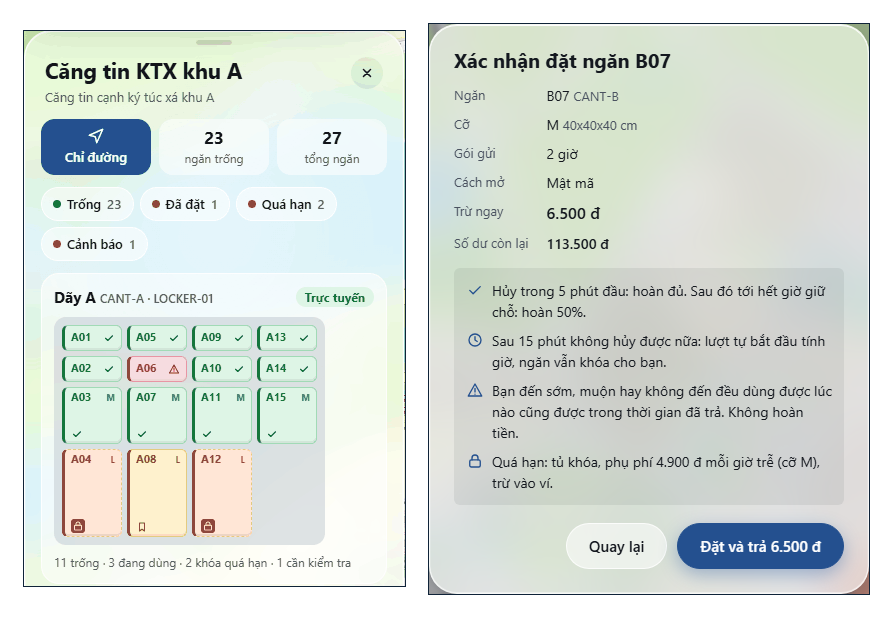
\includegraphics[width=0.9\linewidth,height=0.42\textheight,keepaspectratio]{images/ui-user.png}
\caption{User view of SmartLocker, in which the area panel of the map shows 23 of the 27 slots of a canteen area free
and the slots of bank CANT-A (box LOCKER-01), two of them locked as overdue and one with an open alert, and the booking
confirmation of slot B07 (bank CANT-B, size M, 2-hour plan, PIN) states the 6\,500~VND taken now together with the
refund, automatic start and late-fee rules.}
\label{fig:ui-user}
\end{figure}

\begin{figure}[!htbp]
\centering
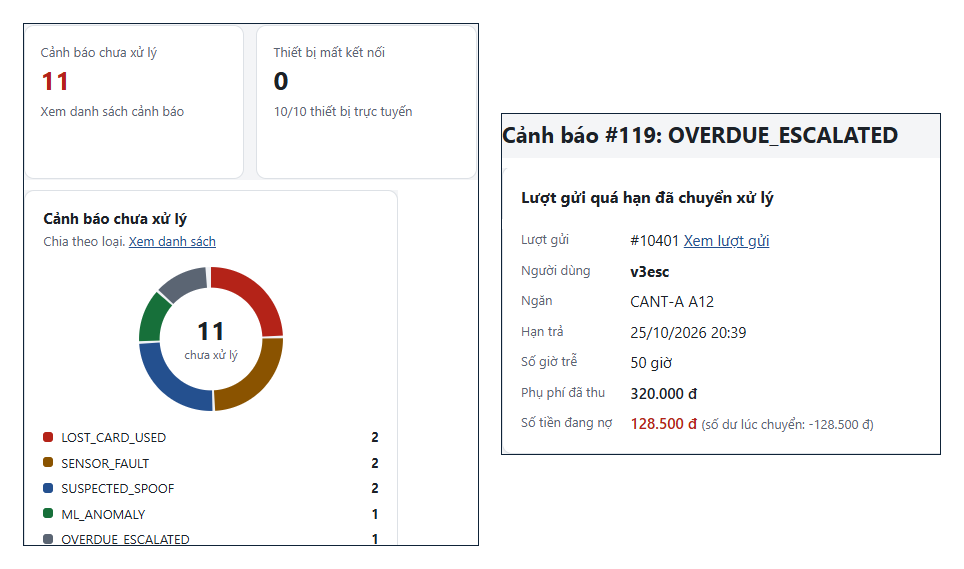
\includegraphics[width=0.9\linewidth,height=0.42\textheight,keepaspectratio]{images/ui-staff.png}
\caption{Staff view of SmartLocker, in which the dashboard tiles show 11 open alerts and no offline device (10 of 10
online) together with the open alerts by type, and alert \#119 (\texttt{OVERDUE\_ESCALATED}) shows a booking in slot
CANT-A A12 that was 50~hours late, with a late fee of 320\,000~VND charged and 128\,500~VND still owed.}
\label{fig:ui-staff}
\end{figure}

\section{Evaluation}
\label{sec:ml}

\subsection{Experimental Setup}

\textit{Dataset.} The risk model is trained on a dataset of 480 rows with five feature columns, the features of
Section~IV-A, and one label column, generated by the group's own seed script \texttt{sql/02\_data\_v1.sql} (2026). No
public dataset was used because none records the door-open time, the weight change and the card of a locker session:
public IoT datasets such as TON\_IoT \cite{moustafa2021toniot} record network traffic and the telemetry of sensors
such as thermostats, fridges and garage doors, but none of these locker fields. The rows are divided into six classes
(NORMAL, FORCED\_OPEN, WRONG\_USER, OVERDUE, ITEM\_LEFT and SUSPECTED\_SPOOF) of 80 rows each. Because the prototype
box has neither a door sensor nor a load cell, the sessions are synthetic: the script generates them from simple
per-class patterns, for example no valid card, a long door time and several unlock events for a forced opening, or a
positive weight change for an item left behind. Wrong-user sessions are produced by exactly the same formulas as
normal ones, since the telemetry of a wrong user is that of an ordinary visit; the two classes differ only in the row
index that the formulas take as input.

\textit{Protocol.} Four Weka classifiers with default parameters were compared: Random Forest \cite{breiman2001rf},
J48 (C4.5) \cite{quinlan1993c45}, Naive Bayes \cite{john1995nb} and IBk with $k = 5$ \cite{aha1991ibl}. Each was
evaluated by stratified 10-fold cross-validation \cite{kohavi1995cv} (seed 42) on the six-class problem and on a binary
NORMAL-versus-ABNORMAL problem, which measures the decision taken by the risk score and is not deployed. Training time
is the median of 11 builds and inference time the mean over $20 \times 480$ predictions after a warm-up, both repeated
in three runs. The experiments ran on an Intel Core i5-11400H laptop (2.7~GHz, 6 cores, 16~GB RAM, 64-bit Windows~11)
with Oracle JDK 1.8.0\_202 and Weka 3.8.6; the server measurements of Section~\ref{sec:latency} used Tomcat 9.0.113 (JDK
1.8.0\_171) and SQL Server 2022 on the same machine. The code counts of Section~V, the tests of Section~\ref{sec:functional} and these measurements refer to commit
\texttt{\measurecommit} of the project repository; the classifier results, the replayed scenarios and the response times
were measured on 30 October 2026, and the rule engine, the risk scorer and the device API they exercise were checked to
be unchanged in that commit.

\subsection{Classification Results}

We report weighted averages over the six classes and over the binary task, so that the deployed model and the risk
decision can be compared on the same folds. IBk achieves the highest weighted F1, 0.977 for six classes and 0.975 for
the binary task (Fig.~\ref{fig:mleval}a), followed by Random Forest (0.948 and 0.939), while Naive Bayes is the weakest
model in the six-class setting (0.778); accuracy, precision and recall of every model are listed in
Table~\ref{tab:ml} in the appendix. All four models are inexpensive enough for online scoring. In the six-class
setting, Random Forest trains in about 36 to 38~ms and scores a session in 12 to 15.5~$\mu$s, whereas IBk requires
essentially no training (under 1~ms) and scores a session in 15 to 17~$\mu$s (ranges over the three runs). The low
computational overhead confirms that telemetry classification can be executed on each incoming session without
degrading server throughput.

\begin{figure}[!htbp]
\centering
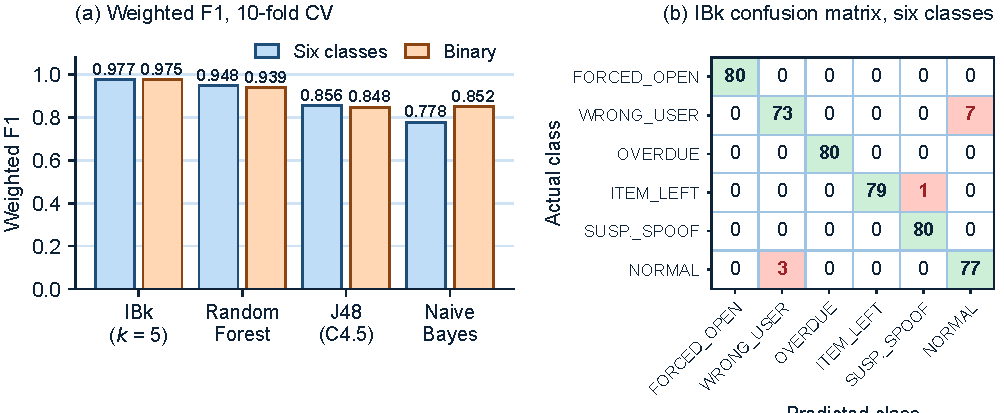
\includegraphics[width=\linewidth,height=0.4\textheight,keepaspectratio]{images/ml-eval.pdf}
\caption{Cross-validation results on the 480 synthetic sessions, with the weighted F1 of the four Weka classifiers
for the six-class and the binary task in (a) and the confusion matrix of IBk for the six-class task in (b), where 10 of
its 11 errors lie between WRONG\_USER and NORMAL.}
\label{fig:mleval}
\end{figure}

\subsection{Discussion}

Per class, the deployed IBk model classifies all 80 FORCED\_OPEN and OVERDUE sessions correctly (F1 1.000), all 80
SUSPECTED\_SPOOF sessions and 79 of 80 ITEM\_LEFT sessions (F1 0.994 each, the remaining ITEM\_LEFT session being
labelled SUSPECTED\_SPOOF), because every abnormal class except WRONG\_USER alters at least one feature in a
characteristic way. The other 10 of its 11 errors involve WRONG\_USER and NORMAL: 7 wrong-user sessions are labelled
NORMAL and 3 normal sessions WRONG\_USER (F1 0.936 and 0.939, Fig.~\ref{fig:mleval}b). Random Forest shows the same
pattern (17 and 8 sessions). This follows from the construction of the data rather than from an empirical observation:
a valid card of another person produces the telemetry of a normal visit, and the residual separation is an artefact of
the row index in the generator. In the binary setting, Naive Bayes classifies every normal session correctly but
labels 80 of the 400 abnormal sessions as NORMAL.

The design does not rest on these scores. Wrong-user access is a question of \emph{identity}, answered exactly by
rule~5, which compares the card owner with the booking owner; lost cards and spoofed remote opens are likewise decided
from the card status and the command table. The learned model is only a secondary signal for unusual combinations of
door time, weight and stay time, and its alerts carry the source ML so that operators treat them with caution
\cite{sommer2010outside}. Because the data are synthetic, the scores above show only that the pipeline works and where
telemetry runs out; they do not predict how the model will behave at a real box, and the risk score should be trusted
only after it has been retrained and checked on labelled real sessions (Section~\ref{sec:limits}). By decoupling
identity verification from numerical feature scoring, the system ensures that physical access rights are strictly
enforced regardless of telemetry variations.

\subsection{Functional Testing}
\label{sec:functional}

\textit{Unit and integration tests} (TestNG). The suite contains 83 test methods in 14 classes. They cover the rule
engine (14 tests), the risk scorer, pricing in Java and its agreement with SQL, the audit hash chain, the device
heartbeat, automatic check-in, phone-tap tokens, pick-up and bank-assignment rules, the access-session list, password
and key hashing, e-mail templates, card confirmation links and box messages. In the final run on commit \texttt{\measurecommit},
all 83 passed and none was skipped. Execution of the complete test suite required approximately two minutes against the
integration test database, confirming that all system components operate in accordance with design specifications.

\textit{API scenarios} (Postman/newman). Eighteen scenarios cover PIN, phone, card and fingerprint access, lost cards,
wrong keys, bodies and codes, the five-try lockout, no-show, overdue lock, top-up, cancellation, escalation, extension
and repeated opens. The first run failed one assertion: with two banks that both contain a slot A01, a session upload
returned HTTP 500 because the slot was looked up by box and slot code only. The server now resolves it by bank code or
by the command's slot and otherwise rejects the session as \texttt{AMBIGUOUS\_SLOT}. Every later run (2~min 27~s, run
of 30 October 2026) executed 221 requests and 472 assertions without a failure.

\textit{Detection scenarios.} A device simulator sends heartbeats, credentials and session uploads signed with the key
of the real box LOCKER-01, and the database is inspected after each scenario (Table~\ref{tab:scen}). All six scenarios
produced the expected label, although two required an adjustment. In the first \emph{remote} run, the simulator
stamped the session in whole seconds, earlier than the command created within the same second, and both sessions were
therefore flagged as spoofed. Since a box clock that lags the server would cause the same false alarm, the rule now
accepts a session stamped up to 60~s before its command, and a rule-engine test covers this window. The simulator's
own \emph{checkin} case sent only a heartbeat, which no longer checks a booking in; the PIN was therefore sent to
\texttt{/api/device/auth}, as the real box does.

\begin{table}[!htbp]
\renewcommand{\arraystretch}{1.1}
\centering
\small
\caption{Detection Scenarios Replayed through the Device API}
\label{tab:scen}
\begin{tabular}{l >{\raggedright\arraybackslash}p{4.6cm} >{\raggedright\arraybackslash}p{3.4cm} >{\raggedright\arraybackslash}p{5.5cm}}
\hline
Scenario & Input & Expected & Observed \\
\hline
heartbeat & 6 heartbeats 10~s apart, then silence & DEVICE\_OFFLINE in 90 to 105~s & \texttt{OFFLINE} and alert 104.6~s after the last heartbeat \\
remote    & staff remote open; the box reports it with the command id, then replays it & STAFF\_OPEN; replay SUSPECTED\_SPOOF & no alert, command \texttt{DONE}; replay \texttt{SUSPECTED\_SPOOF} \\
spoof     & remote session with a command id never issued & SUSPECTED\_SPOOF & \texttt{SUSPECTED\_SPOOF} \\
lostcard  & card reported lost, then used at the box & LOST\_CARD\_USED & \texttt{LOST\_CARD\_USED}; card in the blocked list \\
checkin   & reservation, then its PIN sent to \texttt{/api/device/auth} & UNLOCK, CHECK\_IN & booking \texttt{ACTIVE}, slot \texttt{OCCUPIED}, no alert \\
sensor    & weight change of $-5000$~g (range $-200$ to 20\,000~g) & SENSOR\_FAULT & slot \texttt{MAINTENANCE}; existing ticket kept \\
\hline
\end{tabular}
\end{table}

\subsection{Server-Side Response Time}
\label{sec:latency}

The real box was not connected when the server times were measured, so the values in Table~\ref{tab:latency} cover
only the server processing of the device API: 30 requests per endpoint were sent with curl from the same laptop after
one warm-up request, which excludes Wi-Fi, credential reading and servo movement. The PIN requests used the valid PIN
of an active booking with intent \texttt{ASK}, which the server answers with the ``A: Open / B: Checkout'' choice without
modifying any data.

\begin{table}[!htbp]
\renewcommand{\arraystretch}{1.1}
\centering
\small
\caption{Server-Side Response Time of the Device API (localhost, 30 Requests Each, ms)}
\label{tab:latency}
\begin{tabular}{l c c c c c}
\hline
Request & Mean & Median & p95 & Min & Max \\
\hline
Heartbeat (\texttt{/api/health})                   & 5.9  & 6.0  & 6.8  & 4.6  & 7.3 \\
PIN at the box (\texttt{/api/device/auth})         & 17.0 & 15.7 & 19.0 & 14.1 & 48.0 \\
PIN on the phone page (\texttt{/api/kiosk/unlock}) & 31.1 & 16.2 & 96.0 & 13.4 & 102.7 \\
\hline
\end{tabular}
\end{table}

Every request was answered within about 0.1~s, with a mean of 6 to 31~ms per endpoint, showing that server processing
is negligible compared to physical device delays. A phone-page open also waits for the next heartbeat of the box, which
comes every 3~s. In a separate session with the box online, 20 openings from the phone page took 1.67~s on average
from sending the PIN until the door opened. Most of this delay is the wait for the next heartbeat, 1.5~s on average,
and the server processing time is only a small part of it. The end-to-end time of the other opening methods has not
been measured yet.

Wrong PINs 1 to 4 at the box were answered with 4 down to 1 attempts left. The fifth wrong PIN started a 120~s lock
that also refused the valid PIN (\texttt{LOCKED\_OUT}), and the valid PIN was accepted again 125.5~s after the lock
started. Offline detection uses a 90~s timeout checked every 15~s, so a silent box should be marked \texttt{OFFLINE}
90 to 105~s after its last heartbeat. The heartbeat scenario measured 104.6~s, and four earlier offline alerts of the
same box took 97 to 98~s. One more alert took 110~s because the application was reloaded during the wait, and one alert
raised while the server was stopped is not counted.

\subsection{Limitations}
\label{sec:limits}

The box has no door sensor or load cell and does not yet upload sessions, so every session comes from the device
simulator or the seed data. The training data are synthetic as well, with simple class patterns and shared formulas
for wrong-user and normal sessions, so the cross-validation scores are optimistic and say little about real use; a
transfer test on about 100 labelled device sessions is implemented but could not be run. The classifier results are
therefore exposed to sampling bias and lab-only evaluation, two of the ten pitfalls of learning-based security systems
listed by Arp et al. \cite{arp2024pitfalls}, because every session is synthetic and none comes from a deployed box.
Physically, only one slot has
a lock, and the other banks belong to demo devices. Transport security remains basic: forms carry no CSRF token (only
the \texttt{SameSite=Lax} cookie), Tomcat serves plain HTTP, HTTPS comes only from a Cloudflare tunnel, and the
firmware does not verify the server certificate (\texttt{setInsecure}).

\section{Conclusion}

This paper presented SmartLocker, a locker rental system with online reservation, size-based pricing, four opening
methods and an ESP32 box that delegates every decision to the server. Its main contribution is a priority-ordered rule
tier over telemetry and server context, completed by a credential lockout, offline detection, overdue locking with
escalation and a hash-chained audit log; every replayed detection scenario produced the expected label, and the server
answered device requests within about 0.1~s. The classifier comparison shows why the rules come first: even the best
model, IBk with a weighted F1 of 0.977 on synthetic data, made almost all of its errors between wrong-user and normal
sessions, whose telemetry is the same. Identity cases such as a wrong user, a lost card or a spoofed remote open are
therefore decided by rules, and the machine-learning score should serve only as a secondary signal for unusual door,
weight and stay patterns once it has been trained and checked on real sessions. Future work will add a reed switch and
a load cell with session upload, collect and label real sessions to train and evaluate the model, time every opening
method end to end, lock several slots physically, and add CSRF tokens and certificate verification on the box.

\appendix[Full Cross-Validation Results]

This appendix provides the complete classification metrics for all evaluated models. The weighted averages of the four
classifiers summarised in Fig.~\ref{fig:mleval}a are listed in Table~\ref{tab:ml}. Each model was evaluated under
identical 10-fold cross-validation folds on the 480 synthetic telemetry sessions. The binary task measures the
distinction between normal and anomalous access sessions, reflecting the decision boundary of the risk score.

\begin{table}[!htbp]
\renewcommand{\arraystretch}{1.1}
\centering
\small
\caption{10-Fold Cross-Validation Results (Weighted Averages)}
\label{tab:ml}
\begin{tabular}{l c c c c c c}
\hline
 & \multicolumn{4}{c}{Six classes} & \multicolumn{2}{c}{Binary} \\
Model & Accuracy & Precision & Recall & F1 & Accuracy & F1 \\
\hline
Random Forest & 0.948 & 0.949 & 0.948 & 0.948 & 0.938 & 0.939 \\
J48 (C4.5)    & 0.856 & 0.857 & 0.856 & 0.856 & 0.831 & 0.848 \\
Naive Bayes   & 0.779 & 0.778 & 0.779 & 0.778 & 0.833 & 0.852 \\
IBk ($k=5$)   & 0.977 & 0.978 & 0.977 & 0.977 & 0.975 & 0.975 \\
\hline
\end{tabular}
\end{table}

\section*{Acknowledgment}

The authors thank FPT University for supporting this course project. The authors also thank the course instructors and
reviewers for their constructive feedback on the system design and evaluation. During the preparation of this paper,
the authors used the generative AI assistant Claude (Anthropic) to edit and shorten the English text, to check the
\LaTeX{} source, and to draw the diagrams of Fig.~\ref{fig:arch} to Fig.~\ref{fig:flow} and the chart of
Fig.~\ref{fig:mleval}. The design, implementation, experiments and all reported measurements are the authors' own.
The authors reviewed and edited every AI-assisted part and take full responsibility for the content of this paper.

\bibliographystyle{IEEEtran}
\bibliography{smartlocker-refs}

\end{document}
